\begin{markdown}
#30天 LaTeX 挑戰 Day 20 Ti*k*Z

--------

##可用的選項

TikZ 提供了大量的可自定義的選項,供使用者畫出自己想像中的圖片

###顏色

顏色可以利用 draw 來決定

```latex
\draw[draw = blue] (0,0)--(5,0);
\draw[draw = red] (0,-1)--(5,-1);
\draw[draw = yellow] (0,-2)--(5,-2);
```

如果要填色,可以利用 fill 來填滿顏色,如果目前的圖形不是封閉圖形,那會自動變成封閉圖形

###粗細

粗細可以利用 line width 來決定

```latex
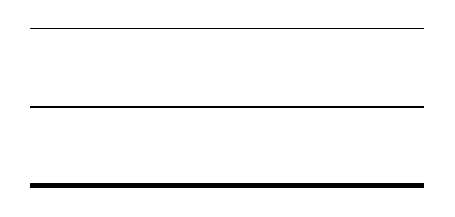
\begin{tikzpicture}
\draw (0,0)--(5,0);
\draw[line width = 1pt] (0,-1)--(5,-1);
\draw[line width = 2pt] (0,-2)--(5,-2);
\end{tikzpicture}
```

TikZ 的預設值是 0.4pt

###箭頭

可以利用 > 與 < 來指定箭頭的形式

```latex
\begin{tikzpicture}
\draw[-] (0,0)--(5,0);
\draw[<-] (0,-1)--(5,-1);
\draw[->] (0,-2)--(5,-2);
\draw[<->] (0,-3)--(5,-3);
\draw[|->] (0,-4)--(5,-4);
\draw[|<->|] (0,-5)--(5,-5);
\draw[|-|] (0,-6)--(5,-6);
\draw[->|] (0,-7)--(5,-7);
\draw[>->>] (0,-7)--(5,-7);
\end{tikzpicture}
```

上圖是一些示範

###預定義好的樣式

TikZ 也有預先定義好一些樣式,讓我們可以使用

```latex
\begin{tikzpicture}
\draw[dotted] (0,0)--(5,0);
\draw[densely dotted] (0,-1)--(5,-1);
\draw[loosely dotted] (0,-2)--(5,-2);
\draw[dashed] (0,-3)--(5,-3);
\draw[densely dashed] (0,-4)--(5,-4);
\draw[loosely dashed] (0,-5)--(5,-5);
\end{tikzpicture}
```

###平移、縮放與旋轉

可以利用 shift 來達成平移的效果

```latex
\begin{tikzpicture}
\draw (0,0) rectangle (1,1);
\draw[shift={(2,0)}] (0,0) rectangle (1,1);
\draw[shift={(2,2)}] (0,0) rectangle (1,1);
\draw[shift={(0,2)}] (0,0) rectangle (1,1);
\draw[shift={(-2,2)}] (0,0) rectangle (1,1);
\draw[shift={(-2,0)}] (0,0) rectangle (1,1);
\draw[shift={(-2,-2)}] (0,0) rectangle (1,1);
\draw[shift={(0,-2)}] (0,0) rectangle (1,1);
\draw[shift={(2,-2)}] (0,0) rectangle (1,1);
\end{tikzpicture}
```

* 第二個正方形的左下頂點由 (0,0) 移到了 (2,0)
* 第三個正方形的左下頂點由 (0,0) 移到了 (2,2)
* 第四個正方形的左下頂點由 (0,0) 移到了 (0,2)
* 第五個正方形的左下頂點由 (0,0) 移到了 (-2,2)
* 第六個正方形的左下頂點由 (0,0) 移到了 (-2,0)
* 第七個正方形的左下頂點由 (0,0) 移到了 (-2,-2)
* 第八個正方形的左下頂點由 (0,0) 移到了 (0,-2)
* 第九個正方形的左下頂點由 (0,0) 移到了 (2,-2)

也可以在 shift 前加上 x 或 y 來決定平移的方向,但在這種情況下就不能使用內建的長度單位,需要自行指定

```latex
\begin{tikzpicture}
\draw (0,0) rectangle (1,1);
\draw[xshift=100pt] (0,0) rectangle (1,1);
\draw[xshift=-100pt] (0,0) rectangle (1,1);
\draw[yshift=100pt] (0,0) rectangle (1,1);
\draw[yshift=-100pt] (0,0) rectangle (1,1);
\end{tikzpicture}
```

旋轉則需要利用 rotate

```latex
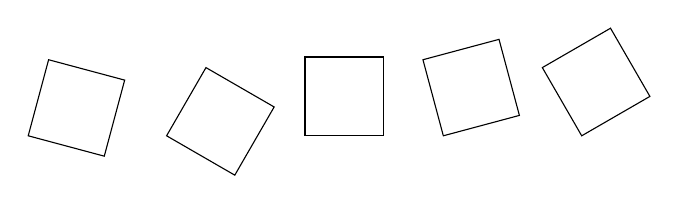
\begin{tikzpicture}
\draw (0,0) rectangle (1,1);
\draw[xshift=100pt, rotate=30] (0,0) rectangle (1,1);
\draw[xshift=50pt, rotate=15] (0,0) rectangle (1,1);
\draw[xshift=-100pt, rotate=-15] (0,0) rectangle (1,1);
\draw[xshift=-50pt, rotate=-30] (0,0) rectangle (1,1);
\end{tikzpicture}
```

\end{markdown}